\chapter{STP Tree Generator}
\label{stp_gen}
We split the application in three parts:
\begin{itemize}
    \item \textbf{Client}: collects STP information and sends it to the server.
        The client also handles piecing together the packets into paths.
    \item \textbf{Server}: saves the data from the clients and combines them into one tree.
    \item \textbf{Parser}: contacts the server to receive the tree and converts it into output format.
\end{itemize}
The intended form of usage is to have multiple clients in the network connecting to one server.
We combine information received from multiple clients to reach a better understanding of the network.

STP uses only local data, which means that bridges have no knowledge of the network, except for their own port states.
Unfortunately for us, this means that it is hard to find connections between bridges.
The only way to obtain this information is to capture packets during the tree build up.

When the client witnesses the message age increasing by one, it assumes that the new root should be prepended to the previous one.
This assumption is unsafe, as this connection cannot be guaranteed, but the risk of making mistakes can be reduced.
Details on this are discussed in the section on unsafe assumptions (Section~\ref{unsafe_assumptions})
Figure~\ref{fig:build_up} shows a rudimentary example of information gained during tree build up.
%TODO: check that the figures don't break any listings
\begin{figure}[p]
    \begin{centering}
        \begin{subfigure}[b]{0.4\textwidth}
            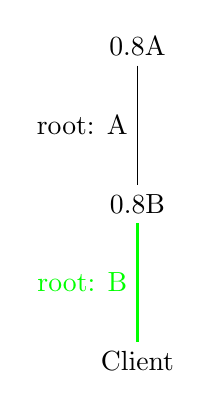
\begin{tikzpicture}
                \node (a) at (4,4) {\switch{0.8}{A}};
                \node (b) at (4,2) {\switch{0.8}{B}};
                \node (client) at (4,0) {Client};

                \draw
                (a) -- node [left] {root: A} ++ (b);

                \draw[green, thick]
                (b) -- node [left] {root: B} ++ (client);

            \end{tikzpicture}
            \caption{B thinks it is root}
        \end{subfigure}
        \hspace{1cm}
        \begin{subfigure}[b]{0.4\textwidth}
            \centering
            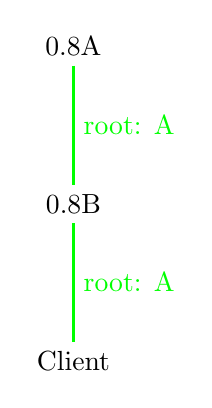
\begin{tikzpicture}
                \node (a) at (4,4) {\switch{0.8}{A}};
                \node (b) at (4,2) {\switch{0.8}{B}};
                \node (client) at (4,0) {Client};

                \draw[green, thick]
                (a) -- node [right] {root: A} ++ (b);
                \draw[green, thick] 
                (b) -- node [right] {root: A} ++ (client);
            \end{tikzpicture}
            \caption{Root information updated}
        \end{subfigure}
    \end{centering}
    \caption{Information gained on STP build up}
    \label{fig:build_up}
\end{figure}

Unfortunately, this works only if the message age increases by one at the same time that the root changes.
For other cases there are simply too many cases to assume a certain change with a reasonable safety.%TODO: source?
Figure \ref{fig:information_lost} shows an example case where the client has to reset its data.
A detailed explanation of how this tool handles incoming STP packets can be found in the section on packet handling (Section~\ref{packet_handling}).

\begin{figure}[p]
    \begin{centering}
        \begin{subfigure}[b]{0.4\textwidth}
            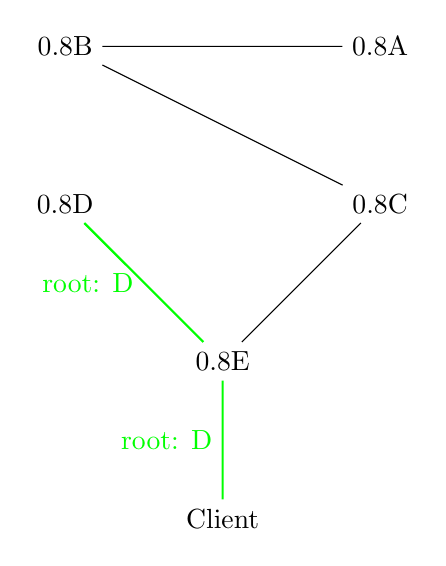
\begin{tikzpicture}
                \node (a) at (6,6) {\switch{0.8}{A}};
                \node (b) at (2,6) {\switch{0.8}{B}};
                \node (c) at (6,4) {\switch{0.8}{C}};
                \node (d) at (2,4) {\switch{0.8}{D}};
                \node (e) at (4,2) {\switch{0.8}{E}};
                \node (client) at (4,0) {Client};
                \draw
                (a) -- (b)
                (b) -- (c)
                (c) -- (e);
                \draw[green, thick]
                (d) -- node [left] {root: D} ++ (e)
                (e) -- node [left] {root: D} ++ (client);
            \end{tikzpicture}
            \caption{Some information known}
        \end{subfigure}
        \hspace{1cm}
        \begin{subfigure}[b]{0.4\textwidth}
            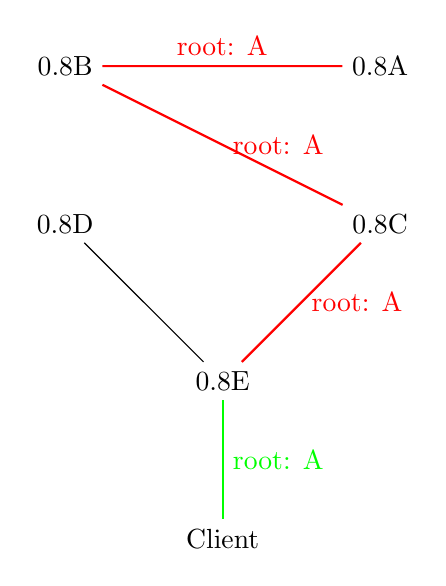
\begin{tikzpicture}
                \node (a) at (6,6) {\switch{0.8}{A}};
                \node (b) at (2,6) {\switch{0.8}{B}};
                \node (c) at (6,4) {\switch{0.8}{C}};
                \node (d) at (2,4) {\switch{0.8}{D}};
                \node (e) at (4,2) {\switch{0.8}{E}};
                \node (client) at (4,0) {Client};
                \draw
                (d) -- (e);
                \draw[green, thick]
                (e) -- node [right] {root: A} ++ (client);
                \draw[red, thick]
                (a) -- node [above] {root: A} ++ (b)
                (b) -- node [right] {root: A} ++ (c)
                (c) -- node [right] {root: A} ++ (e);
            \end{tikzpicture}
            \caption{Previous information lost}
        \end{subfigure}
        \caption{Information lost during tree build up}
        \label{fig:information_lost}
    \end{centering}
\end{figure}

\section{Details}
\subsection{Saving the Data}
\label{data}
%TODO: explain how the sniffer saves data before sending it
%TODO: explain what clearAndAdd does
\subsection{Packet Handling}
\label{packet_handling}
Packets are handled by the Sniffer class.
While most of the function that handles incoming STP packets just skip fields that are not used, here we will discuss the more important parts.
In order to check if the packet is actually an STP packet, we use the Ethernet destination address:
\lstinputlisting[language=C++]{../listings/stp/stpFilter.c}
Where bytes is provided by the required \textit{pcap} callback prototype (see Section~\ref{pcap}: PCAP).
This is computationally more expensive than saving the destination in binary format and comparing memory.
It is however also more readable and a lot easier to change should the need arise.

\textit{Pcap} provides us with a pointer to the binary packet data.
We can go through the packet by incrementing this pointer by set amounts (after skipping to the STP data):
\lstinputlisting{../listings/stp/payload.c}
This repeats for the bridge identifier, as well as other fields.

After the data is extracted from the packet, it is constructed into our custom classes.
We then check if the two bridges (root and first hop) were previously known:
\lstinputlisting{../listings/stp/contained.c}
Concerning the root, knowing whether or not it was previously known is enough.
For the first hop, we also require knowledge about the old message age.

Finally we can update the saved information in the Sniffer:
\lstinputlisting{../listings/stp/update.c}
\subsection{Communication}
\label{communication}
As discussed in the background section (Section~\ref{json}) wer are using JSON for the client server communication.
\subsection{Combining the data}
\label{combining_data}
\subsection{Unsafe Assumptions}
\label{unsafe_assumptions}
\section{Installation \& Usage}
